\begin{figure}[H]
	\centering
	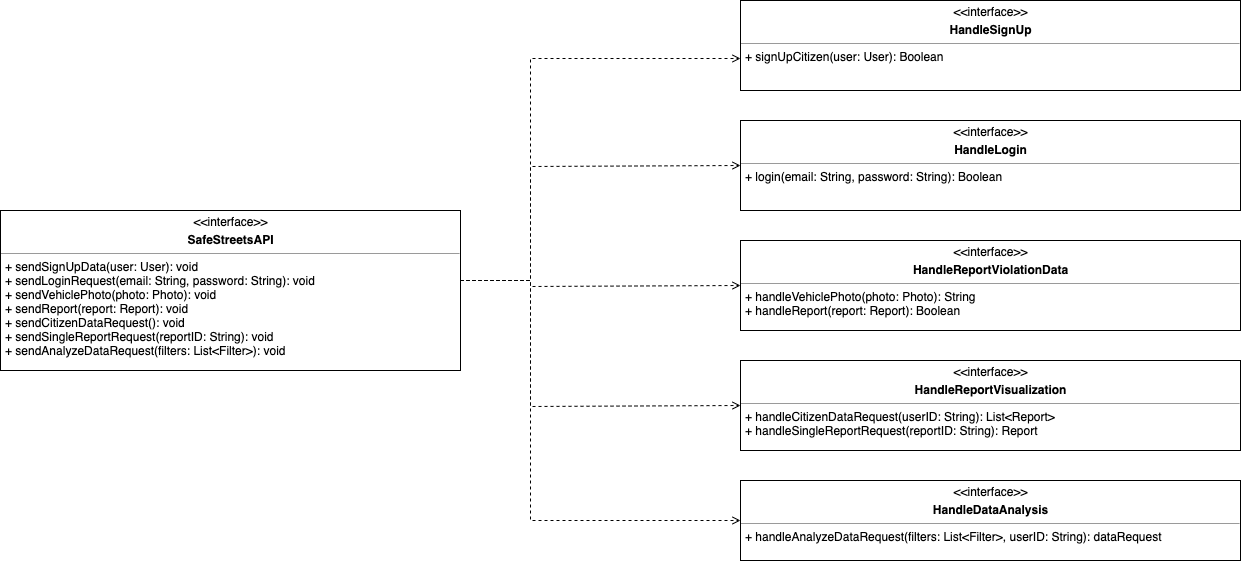
\includegraphics[width=\linewidth]{Images/CitizenComponentInterfaces}
	\caption{Citizen component interfaces.}
\end{figure}
\begin{figure}[H]
	\centering
	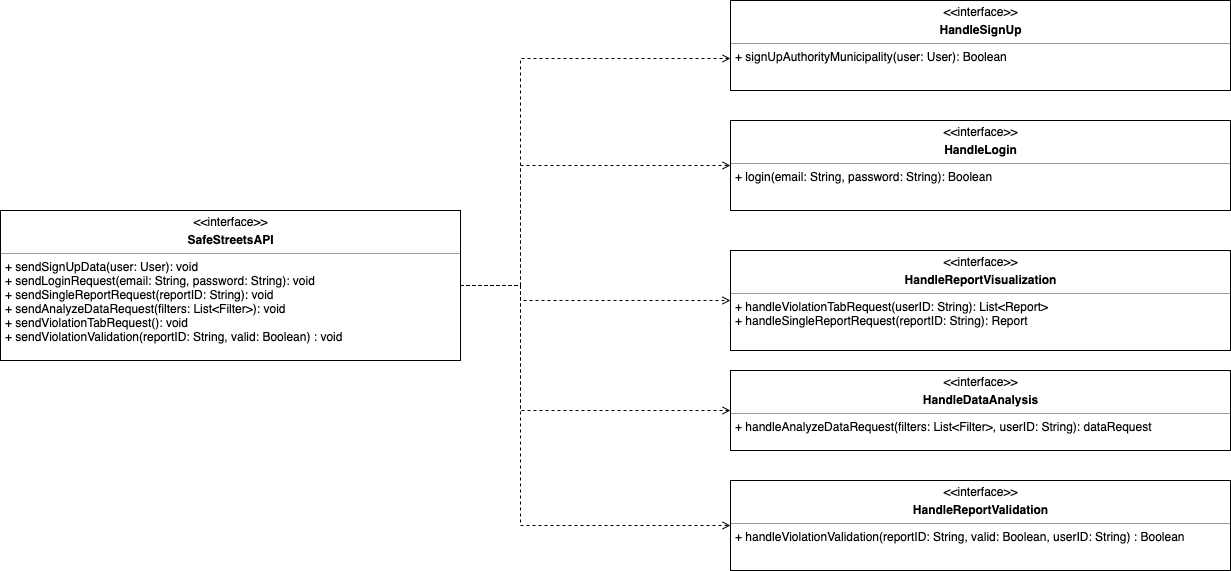
\includegraphics[width=\linewidth]{Images/AuthorityComponentInterfaces}
	\caption{Authority component interfaces.}
\end{figure}
\begin{figure}[H]
	\centering
	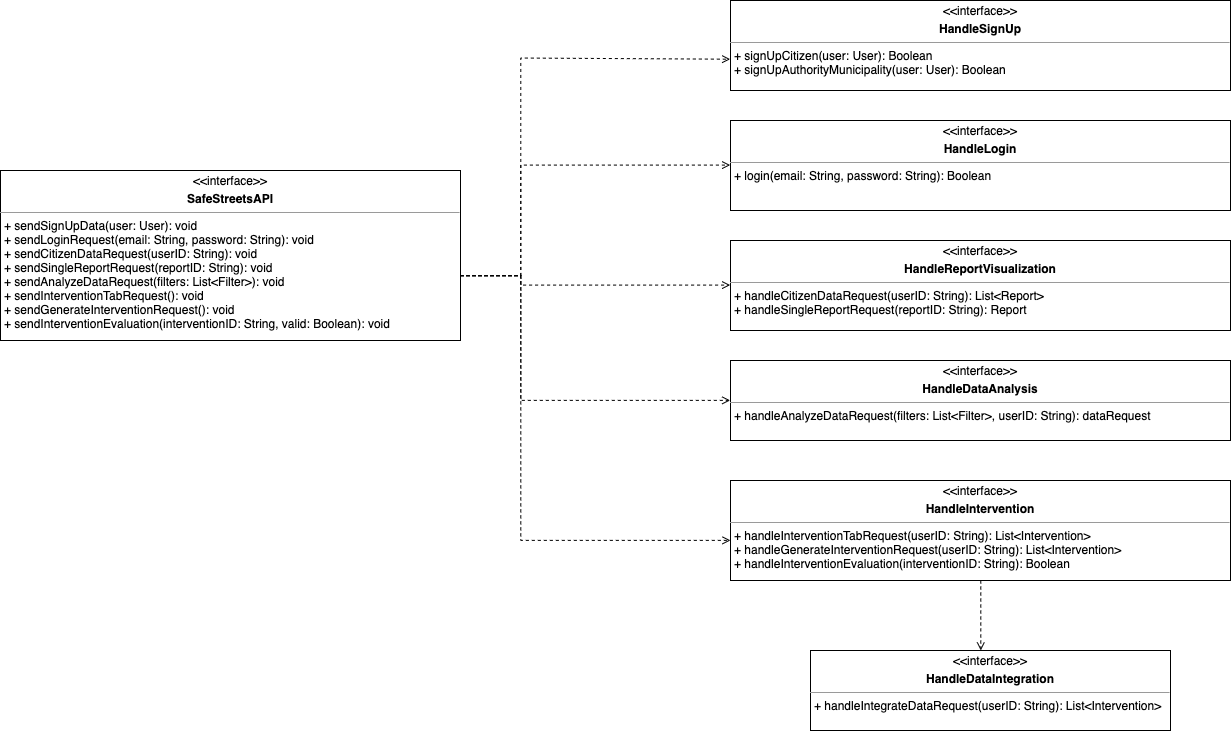
\includegraphics[width=\linewidth]{Images/MunicipalityComponentInterfaces}
	\caption{Municipality component interfaces.}
\end{figure}
The above figures show the component interfaces of the application server that are actually used for each kind of user. The SafeStreetsAPI interface provides all the methods needed to access the services offered by the application server. Each method of this interface is associated by the 'Router' component with an internal handler interface provided by the component responsible of the requested service. Each internal interface handles the incoming requests and communicates with the DBMS for database modification. In the following, a description for each one of these interfaces is provided:
\begin{itemize}
	\item HandleSignUp: this interface is responsible for the sign up of any kind of user; in particular if the user is an authority or a municipality, it verifies its identity by checking their PEC address with external an PEC API.
	\item HandleLogin: this interface is responsible for authenticating the access of a user and establishing a connection session.
	\item HandleReportViolationData: this interface is responsible for recognizing the license plate of incoming vehicle photos, using an external OCR API; it also receives reports from the clients, completes them with metadata and stores them in the databases.
	\item HandleReportVisualization: this interface is responsible for sending all data regarding the reports of a specific citizen user, reports in the jurisdiction of the requesting authority for the violation tab or just just one single report.
	\item HandleDataAnalsysis: this interface is responsible for retrieving data that satisfies the filters of the incoming data analysis requests; for each kind of requesting user it sends back different amount of data for privacy security reasons, in fact both kinds of users can retrieve the location, time and type of violation of the reported transgressor, but only the authorities can retrieve the license plates, whereas citizen cannot.
	\item HandleReportValidation: this interface is responsible for receiving violation validations from authority users and update the database accordingly.
	\item HandleIntervention: this interface is responsible for sending the previously generated reports and generating new interventions when requested by the municipality, and it also receives intervention evaluations to update the database accordingly.
	\item HandleDataIntegretaion: this interface is responsible for retrieving data from the municipality's server and integrate it with data collected by SafeStreets, by inserting 
\end{itemize}